This section will look at different ways of importing or creating city maps in Unity. The purpose of this is to give the agents an environment that more accurately replicates the real world. There are two main ways of doing this. The first option is loading the maps in at runtime. This option would give the agent an unbounded area to navigate around. The second option is to create a Unity asset. This option allows the user to create a 3D model of the environment and load the object into the scene at compile time.  
\subsection{Unity Map SDKs}
There are several different Map SDKs available for Unity. The advantage of using an SDK over an asset is that it allows the user to navigate any place. As the agent navigates around, new areas of the map will be loaded. Another advantage is that the maps are updated and can provide real information such as traffic congestion. A disadvantage is that these maps need to be download at runtime. This requires access to the internet and can be slow to load. Another disadvantage is that these services are subscription-based. This means that there is a limit to the number of requests that can be made \cite{}.

\subsubsection{Google Maps Unity SDK}

Google Maps Unity SDK contains several developer tools which allow the user to create mobile games with real-world locations\cite{google_maps_sdk_platform}. The advantage of using this SDK is that it provides additional tools such as the ability to extract place IDs as well as the name of geographic features. The SDK also includes real-world features from particular locations. (Appendix~\ref{Appendix_Maps} - Figure~\ref{figure:maps:GoogleMapsSDK_Liberty}). The disadvantage with the Google Maps SDK is that it currently only supports mobile applications. The simulator is primarily designed to run on a computer so this SKD would therefore not work for this project. 

\subsubsection{MapBox Unity SDK} 
The MapBox Unity SDK is a toolbox that can be used to create worlds with continuous road networks, points of interests and street labels. It also can use satellite images to create realistic terrain. The advantage of the MapBox SDK is that it is free and easy to set up. The disadvantage is that the generated textures do not look as good as other map options. There are also some missing buildings as can be seen from Figure~\ref{maps:figure:MapBox}. MapBox does allow the users to modify the maps online, but this has to be approved before the maps are updated.  

\subsubsection{Wrld3D Unity SDK} 
Wrld3D Unity SDK is a dynamic 3D mapping platform that can replicate indoor and outdoor environments. Similar to the SDK created by Google, famous landmarks and features are recreated. The SDK comes with a variety of different APIs. These include,  for example, select and highlight buildings, enter and exit indoor maps and visualise the transport network. As can be seen from Figure~\ref{maps:figure:Wrld3D}, the applied textures look better than the textures provided from the MapBox SDK (Figure~\ref{maps:figure:MapBox}). Wrld3D costs 20 USD per months making it one of the more expensive options. The maps are however more visually appealing than the other options. In addition, the maps have smoother and more accurate surfaces making it easier for the simulation, compared to for example the Google 3D maps loaded into Blender (Figure~\ref{maps:figure:GoogleMaps}).

\begin{figure}[!htbp] 
\centering
\begin{minipage}{.45\textwidth}
\centering
\begin{subfigure}{\textwidth}
        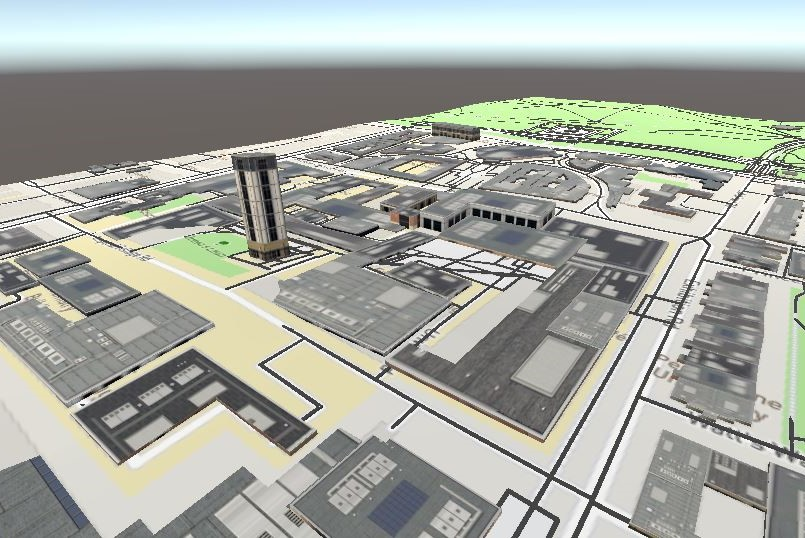
\includegraphics[width=\linewidth, left]{06_Implementation/00_Maps/Images/MapBox1Cropped.JPG}
        \caption{Imperial Campus loaded into Unity using the MapBox SDK. All objects have been given an arbitrarily texture. Also, the building scale is off.}
        \label{maps:figure:MapBox}
    \end{subfigure}
\end{minipage}
\qquad
\begin{minipage}{.45\textwidth}
    \centering
    \begin{subfigure}{\textwidth}
        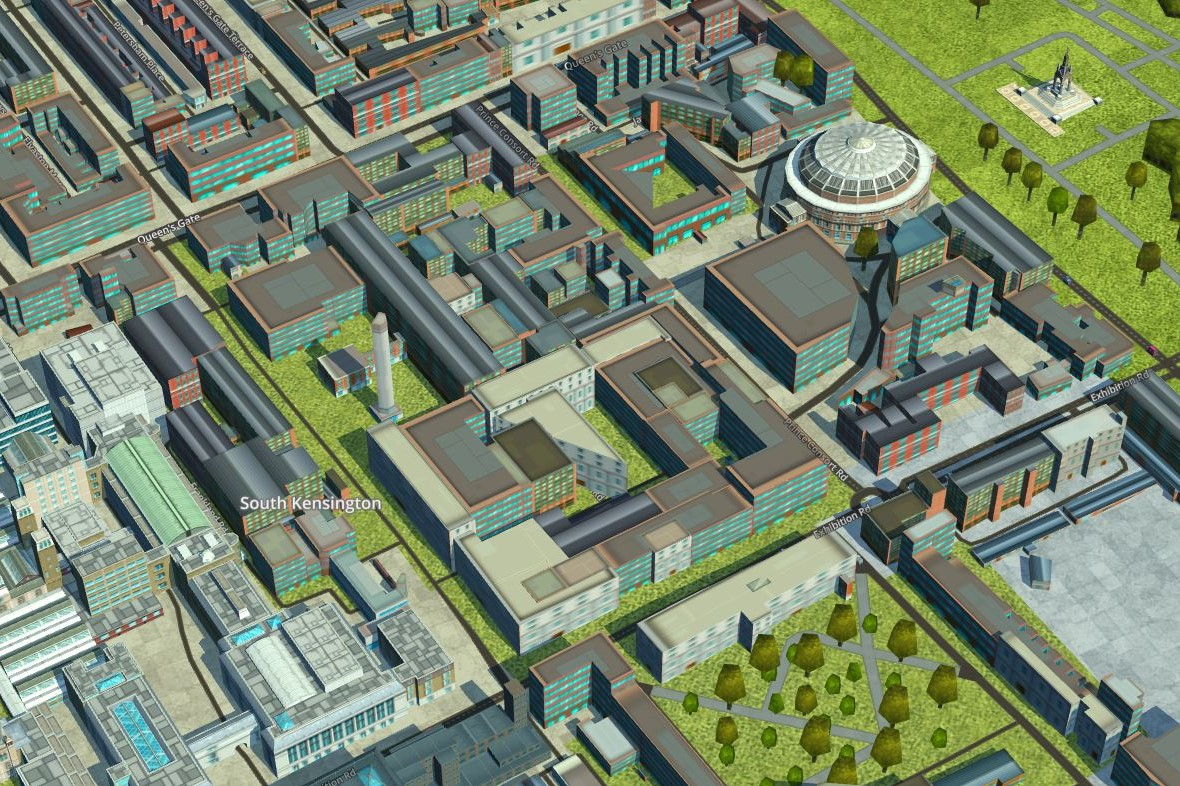
\includegraphics[width=\linewidth, right]{06_Implementation/00_Maps/Images/Wrld3D1Cropped.JPG}
        \caption{Wrld3d has a tool online where you can look at the map before purchasing the SDK subscription. The image is a screenshot from this tool\footnote{\url{https://maps.wrld3d.com/?mapscene=632ba4b}}.}
        \label{maps:figure:Wrld3D}
    \end{subfigure}
\end{minipage}
\end{figure}

\FloatBarrier
\subsection{Unity Map Assets}
Loading map assets into Unity requires more initial work as they require 3rd party tools. An advantage of creating assets is that it gives the user the freedom to modify the maps before importing them into the simulator. Blender is commonly used as a free program for creating and modifying 3D models\cite{MendozaGuevarraEzraThess2020CGEi}(Section~\ref{Blender}). Another advantage is that the maps are loaded at compile-time. This means that the model loads quickly and the simulator does not require access to the internet. The disadvantage is that the agents will be limited to only that environment. Large maps can be computationally hard to render and cause the simulator to lose performance. This is due to the large polygon count which requires more memory and CPU usage. (More information in the User Guide Section~\ref{}). Depending on the method used to create the models, creating better-looking options using Blender can be very time-consuming and requires additional skills to use the tool. 


\subsubsection{OpenStreetMap2World}
OSM2World is an open-source program that takes maps generated by Open Street Map\footnote{\url{https://www.openstreetmap.org/\#map=16/51.4976/-0.1715}} and them into object files which can be loaded into Unity. There are several advantages of using OSM2World to create assets. Firstly, this program is easy to set up and generate object files. The user can either use the GUI or use the CLI. Another advantage is OSM2World creates objects which consist of several layers. These layers are different features the world consists of, for example, roads, junctions, footpaths and buildings. Having these layers allows the user to interact with each of them separately. Users can manually modify these layers on the OpenStreetMap website\footnote{\url{https://www.openstreetmap.org/}}.

The disadvantage of using OSM2World is that it does not allows to render the objects with texture in Unity. It is also difficult to make adjustments to the environment without using another tool like Blender. These adjustments could be updates that the user would like to have for their environment, but are not changes that should be uploaded to the map itself, like adding additional walls to close the area.

\begin{figure}[H]
    \centering
    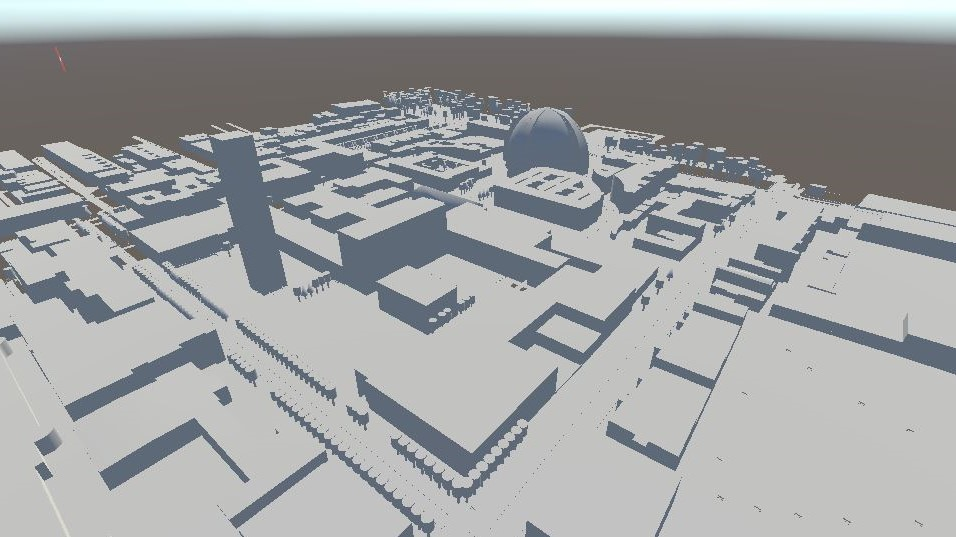
\includegraphics[width=0.65\textwidth]{06_Implementation/00_Maps/Images/OSM1Cropped.JPG}
    \caption{South Kensington Campus created using OpenStreetMap2World loaded into Unity}
\end{figure}

More information on how to create an object file from OpenStreetMap can be found in the user guide~\ref{}.
\subsubsection{BlenderGis}
BlenderGis is an open-source Blender addon that allows users to import GIS (geographic information system) files. The addon includes the option to download a map area from either Google or OpenStreetMaps directly into Blender without having to download the GIS files externally. One advantage of using BlenderGis over OSM2World is that GIS files include the world heightmap. This means that this method can more accurately map the terrain. 

BlenderGIS can also be used to import structures and buildings like OSM2World, and the quality is somewhat similar. This Blender addon also includes the different map layers like OSM2World, but there are not as many options. Different kinds of roads, junctions and so on are all just marked as highway. 

The main advantage of using BlenderGIS over OSM2World is that BlenderGIS allows adding texture to the map. The satellite image is projected onto the map ground, making the scene much more recognisable. There is also a way of projecting the textures onto the buildings. As the satellite images are only taken from above, there is no way to add texture to the sides of the buildings without using a generic front. 

\begin{figure}[H]
    \centering
    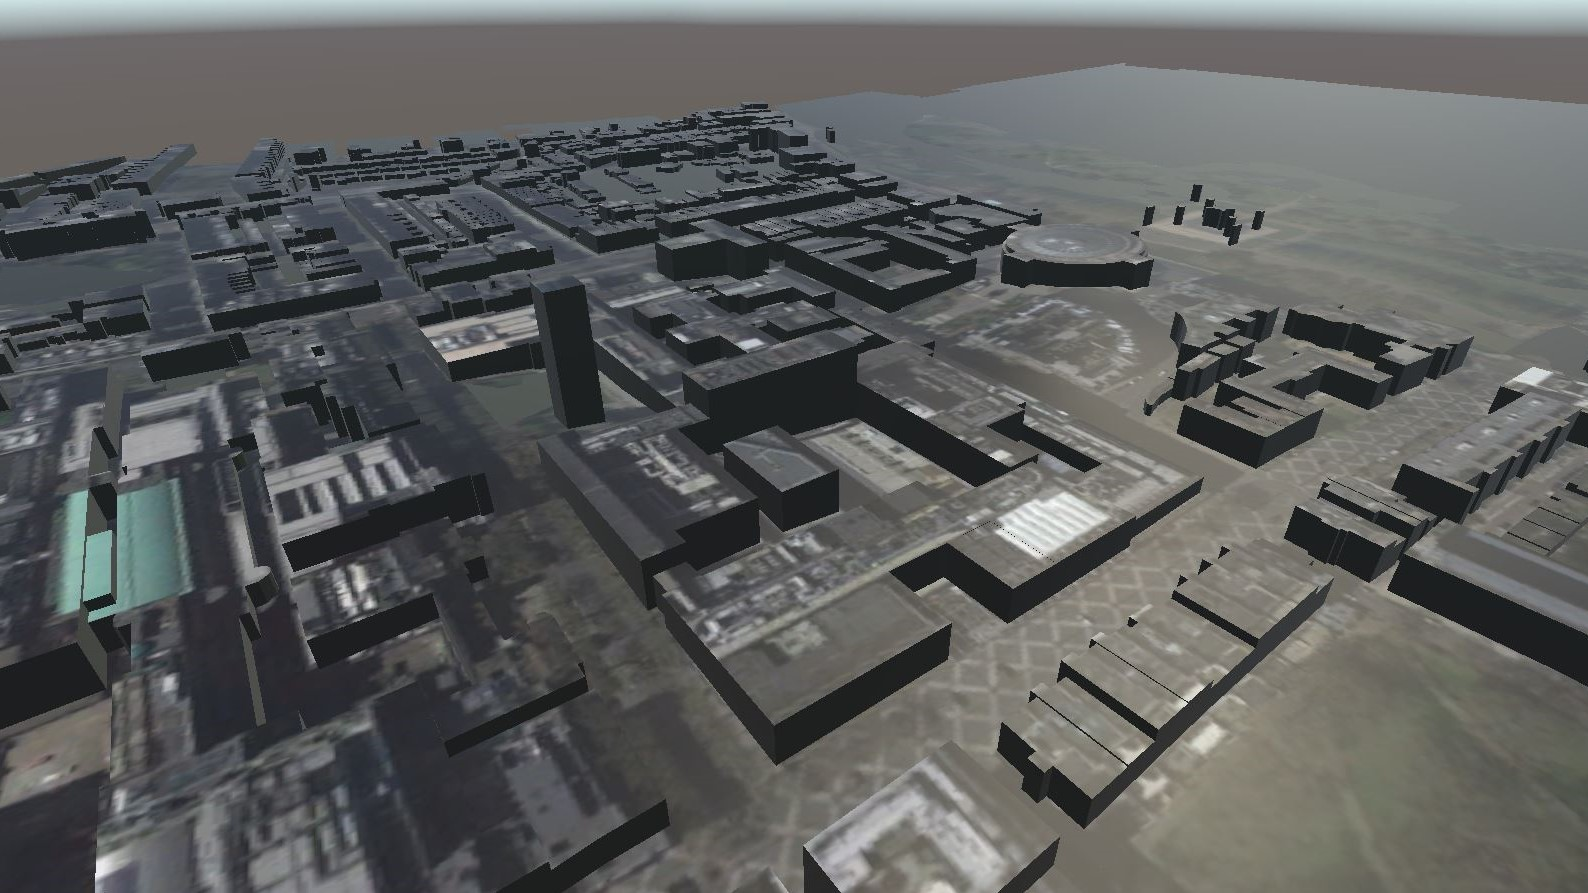
\includegraphics[width=0.65\textwidth]{06_Implementation/00_Maps/Images/BlenderGis1Cropped.JPG}
    \caption{South Kensington Campus created using BlenderGis, then load into Unity. Some buildings are missing and the texture looks quite flat.}
\end{figure}

More information on how to install and use the addon can be found in the user guide (Section~\ref{}).

\subsubsection{Google Maps GPU Intercept}
For personal projects, Google Maps' 3D view can be imported into Blender. These steps are quite convoluted, but the user guide (Section~\ref{}) explains how to do this in more detail. In essence, renderDoc can be used to intercept the data going from Google Chrome to the GPU. This data can then be loaded into Blender by using MapsModelImporter\footnote{\url{https://github.com/eliemichel/MapsModelsImporter}}. This step can take a long time as many polygons have to be loaded. Once the map has been imported into Blender, the user can freely update the model. One update that should be made is to reduce the polygon count. Blender has a tool for this. This is needed as there are several thousand polygons, and this process can remove almost half without a noteworthy difference (Figure~\ref{maps:figure:GoogleMaps}). Finally, the model along with the textures can be exported to Unity. 

The advantage of using this method is that it looks a lot better than the other options. There is also a lot more detail which makes the environment more realistic. This can be useful when training machine learning models as the trained model would not overfit to a perfect environment. 

However, there are several disadvantages to using this method. Firstly, creating maps using this method is a lot more time-consuming. Importing the map into Blender, then exporting it to Unity can take several hours due to a large number of polygons. This method is also a lot more computationally expensive when running in Unity, as each polygon has to be rendered. Secondly, the roads are not even and flat, as cars on the roads are incorporated into the model. This can be smoothed using tools in Blender, but this is once again time-consuming. The last disadvantage is that the model does not include map layers which the other method do. This means there is no way of distinguishing different objects, like buildings, trees and parked cars, apart. 

\begin{figure}[H]
    \centering
    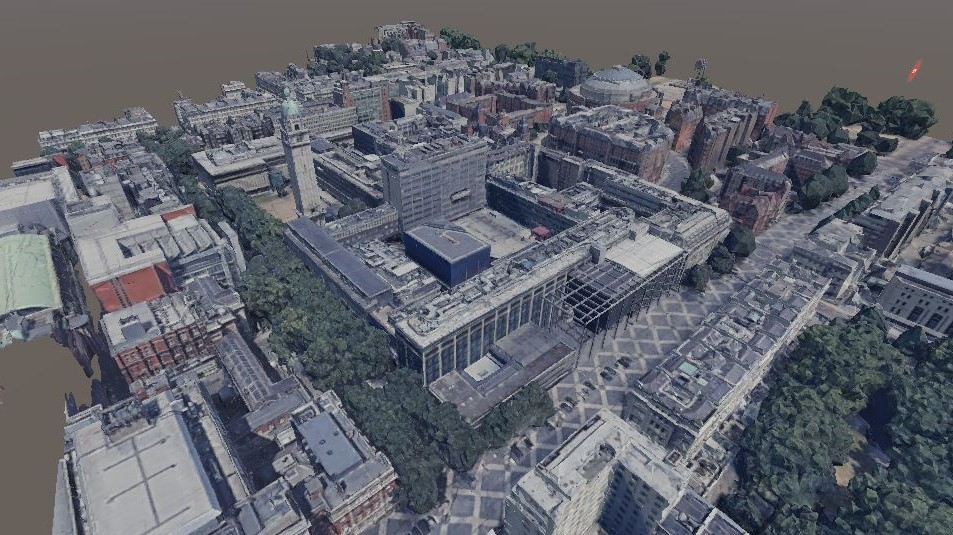
\includegraphics[width=0.7\textwidth]{06_Implementation/00_Maps/Images/Google5Cropped.JPG}
    \caption{South Kensington Campus loaded from Google Maps into Blender, then exported to Unity. Number of polygons reduced by 60\%}
    \label{maps:figure:GoogleMaps}
\end{figure}

\subsection{Conclusion}
For this project using map assets rather than an SDK would be better. As the simulation is about the interaction between different kind of agents, an infinite map is not required. Using an SDK is a good alternative if the specification for the project changed and training agents at several different random locations became more important. The benefit of the faster loading time and not having to rely on an external API at runtime makes loading the environment as a Unity asset the best option. 

In regards to which of the asset methods to go for really depends on the task. For a visual demonstration, the optimal choice would be to overlay the data from Google Maps on top of the height map generated by BlenderGis. This can be seen in Figure~\ref{maps:figure:combined}. This approach would then allow for smooth roads whilst keeping the detail on the buildings and other structures. 

If the visual is not important, using something like BlenderGis would work well. This allows for a layered map as well as providing the terrain height. It is also easy to set up and use. 

\begin{figure}[H]
    \centering
    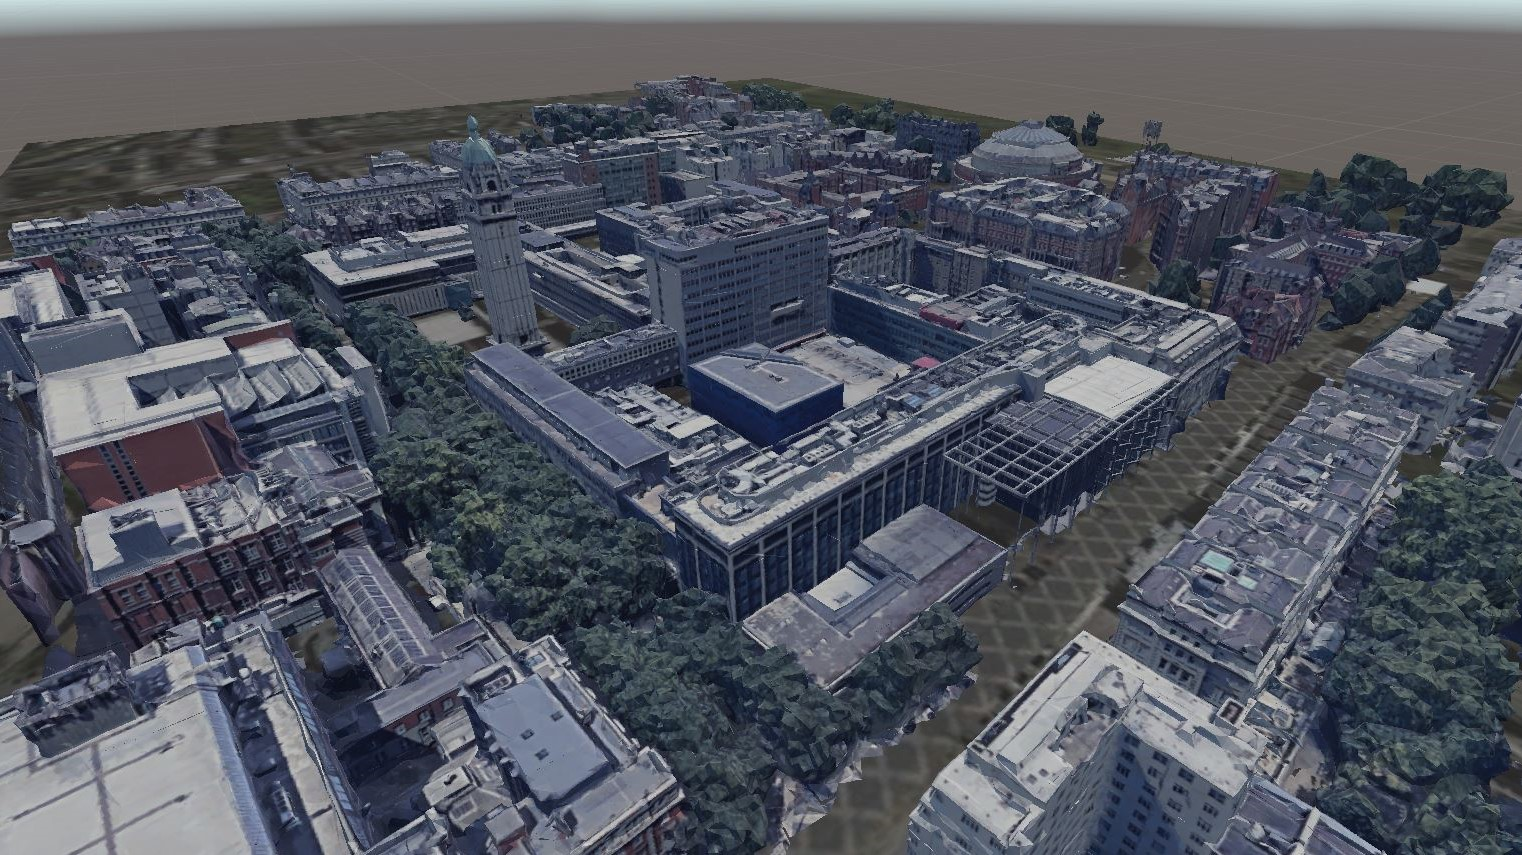
\includegraphics[width=0.7\textwidth]{06_Implementation/00_Maps/Images/CombinedCropped.JPG}
    \caption{BlenderGis and Google maps combined. Allows for smooth roads whilst keeping the aesthetics of the buildings}
    \label{maps:figure:combined}
\end{figure}
